
\section{Evaluation}
\label{sect:exper}

We have implemented and evaluated a prototype of our multi-stage deduplication scheme on a cluster
of dual quad-core Intel Nehalem 2.4GHz E5530 machines with 24GB memory.  
Our implementation is based on Alibaba's Xen cloud platform~\cite{Aliyun,WeiZhangIEEE}.
Objectives of our evaluation are:
1) Analyze the deduplication throughput and effectiveness for a large number of VMs.
%Compare with the data domain approach~\cite{bottleneck08}.
2) Examine the impacts of buffering during metadata exchange.

%\subsection{Experimental setup}

%We are running our deduplication/backup  service on 100 nodes.
%Memory usage is about 150MB space per node during backup and
%the CPU usage is very small during the experiments. 
We have performed a trace-driven study using  a 1323 VM dataset  collected from 
%100 Alibaba Aliyun's cloud nodes~\cite{WeiZhangIEEE}.
a cloud cluster at Alibaba's Aliyun.
% ~\cite{WeiZhangIEEE}.
% and each of machine nodes has 16 cores and 12 disk drives,  hosting  up to 25 VMs. 
For each VM, the system keeps 10 automatically-backed snapshots in the storage while
a user may instruct extra snapshots to be saved.
The backup of VM snapshots is completed within a few  hours every night.
Based on our study of its production  data,  each VM has about  40GB of storage  data usage on average
including OS and user data disk.
Each VM image is  divided into 2 MB fix-sized segments and each segment is divided into 
variable-sized content blocks  with an average size of 4KB.
%variable sizes~\cite{similar94,rabin81} with an average size of 4KB. 
The signature for variable-sized blocks is computed using their SHA-1 hash. 

The seek cost of each random IO request in our test machines is about  10 milliseconds.
The average I/O usage of local storage is controlled about 50MB/second for backup 
in the presence of other I/O jobs. Noted that a typical 1U server can host
6 to 8  hard drives and deliver over 300MB/second. Our setting uses 16.7\% or less 
of local storage bandwidth. 
The final snapshots are stored in a distributed file system built on the same 
cluster. 

The total local disk usage on each machine is about 8GB for the duplicate detection purpose,
mainly for global index. 
Level 1 segment dirty bits identify 78\% of duplicate blocks. For the remaining dirty segments,
block-wise full deduplication removes about additional 74.5\% of duplicates.
The final content copied to the backup storage is reduced by 94.4\% in total.

\begin{figure}
\centering
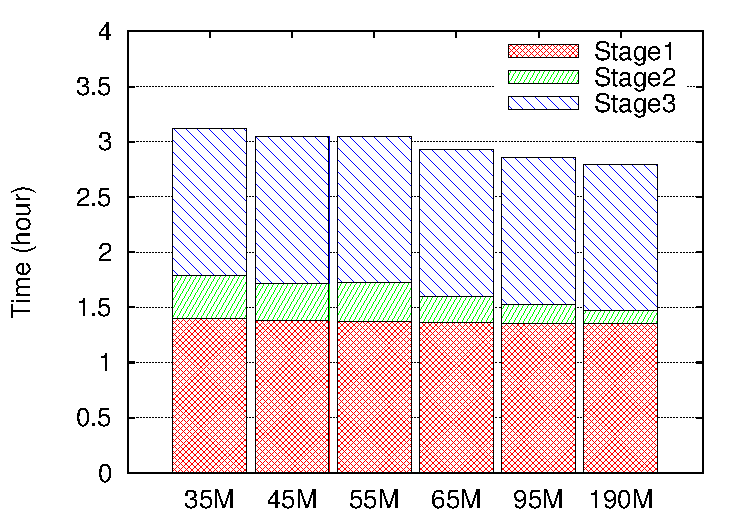
\includegraphics[width=0.4\textwidth]{mem_time.pdf}
\caption{ Parallel time when memory limit varies.}
\label{fig:memory}
\end{figure}

Figure~\ref{fig:memory} shows the total parallel time in hours to backup 2500 VMs on
 a 100-node cluster a  when 
limit $M$ imposed on each node varies.
%  from 20MB to 200MB.
This figure also depicts the time breakdown for Stages 1, 2, and 3. 
%The parallel time includes the first scanning time, 
%of dirty VM segments to generate block fingerprints, data redistribution for request accumulation,
%fingerprint comparison, duplicate summary distribution, and the second scan time for real backup.
The time in Stages 1 and 3  is  dominated by  the two scans of dirty segments,
and final data copying to the backup storage is overlapped with VM scanning.
During dirty segment reading, the average number of consecutive dirty segments is 2.92. 
%Each scan takes about 1.4 hours.
The overall processing time does not have a significant reduction as $M$ increases to 190MB.
The aggregated deduplication throughput is  about 8.76GB per second,
which is the size of 2500 VM images divided by the parallel time. 
The system runs with  a single thread and  its CPU resource usage is 10-13\% of one core. 
The result shows the backup with multi-stage deduplication  for all VM images can be 
completed in about 3.1 hours with 35MB memory,  8GB disk overhead and a small CPU usage.
As we vary the cluster size $p$,  the parallel time does  not change much, and  the aggregated throughput
scales up linearly since the number of VMs is  $25p$. 

Table~\ref{tab:overall} shows performance change when limit $M$=35MB is imposed and
the number of partitions per machine ($q$) varies.
% varies from 100 to 1000.
Row 2 is memory space required to load a partition of global index and detection requests.
When $q=100$, the required memory is 83.6 MB and this exceeds the limit $M=$35MB.  
Row 3 is the parallel time and Row 4 is  the aggregated throughput of  100 nodes.
%The result shows the backup with multi-phase deduplication  for all VM images can be completed in about 3.09 hours
%with the very small resource usage.
Row 5 is  the parallel time for using Option 1 with $p\times q$ send buffers 
described in Section~\ref{sect:arch}. 
When $q$ increases, the available space per buffer reduces and there is a big increase of seek cost.  
The main network usage before performing the final data write is for request accumulation and
summary output. It lasts about 20 minutes and each machine exchanges 
about   8MB of metadata per second with others during that period, which is 6.25\% of the network bandwidth.

\begin{table}[hbt]
\caption{ Performance when $M$=35MB and $q$ varies.}
\begin{center}
\begin{tabular} {|c|c|c|c|c|c|}
\hline \#Partitions ($q$)  & 100 & 250  & 500 &  750 &  1000 \\
\hline Index+request & 83.6 &  33.5 & 16.8 & 11.2 & 8.45 \\
  (MB)           &  &   &  & &  \\

\hline Total Time  & N/A&  3.12 & 3.15 & 3.22 & 3.29 \\
  (Hours)           &  &   &  & &  \\
%\hline Throughput/node & N/A&  85MB/s& 90M & 87 & 81 \\
\hline Throughput GB/s& N/A&  8.76 & 8.67 & 8.48 & 8.30 \\
\hline Total time & N/A&  7.8& 11.7 & 14.8 & 26 \\
  (Option 1)           &  &   &  & &  \\
\hline
\end{tabular}
\end{center}
\label{tab:overall}
\end{table}

%\begin{verbatim}
%memory
%#partitions/node	50	100	250	275	300	450	500	750	1500	2000
%Memory meta data 0.161	0.0805	0.0322	0.029272727	0.026833333	0.017888889	0.0161	0.010733333	0.005366667	0.004025
%Global index 0.115	0.0575	0.023	0.020909091	0.019166667	0.012777778	0.0115	0.007666667	0.003833333	0.002875
%Seek (Step 1) 0.0212962960.0425 0.106 0.117 0.127777778	0.191666667	0.212962963	0.319444444	0.638888889	0.851851852
%Seek Option 2: 6.388888889	12.77777778	31.94444444	35.13888889	38.33333333	57.5	63.88888889	95.83333333	191.6666667	255.5555556
%Total time 3.059031718	3.078670034	3.131061779	3.137163671	3.141047877	3.313871832	3.296994302	3.377385758	3.689876824	3.901831421
%throughput  per node 0.090805785	0.090226551	0.088716799	0.088544242	0.088434748	0.083822728	0.084251822	0.082246387	0.075281044	0.07119164
%
%\end{verbatim}

%\begin{figure}
%  \centering

%  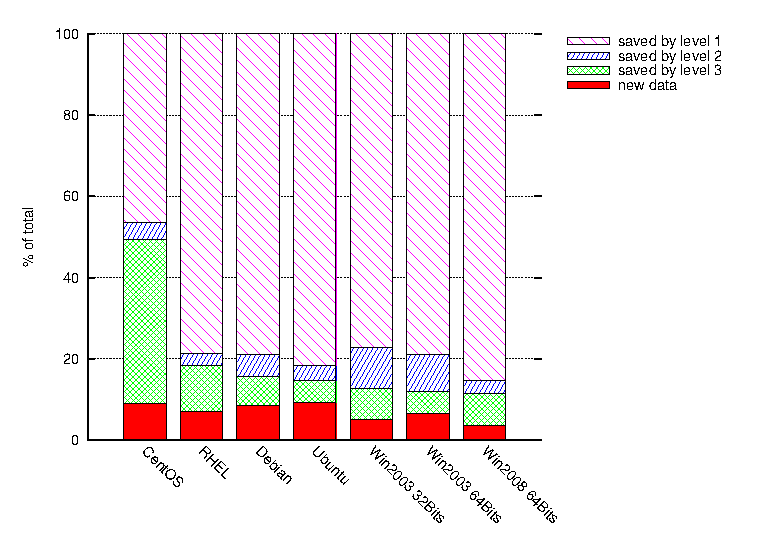
\epsfig{file=images/3level_os.eps, width=3.5in}
%  \caption{Impact of 3-level deduplication for OS releases.}
%  \label{fig:oscds}
%\end{figure}

%To see the impact of multi-level deduplication on different OS releases,
%Some of  OS disks are modified frequently and in some cases,  users even store a large amount of user data on


\comments{
%\begin{verbatim}
%q= is chosen between 500 or 100
Memory limit:   20 35M   50M  75M  100M  200M
req buf	        15M 30M   40M  60   90M     180M
q:           450     275    275   275 275   
Time:         3.1  2.9  2.86  2.84 2.834  2.823
stage 1      1.53    1.4   1.38  1.37 1.36 1.35
stage 2	     0.23    0.17 0.15   0.15 0.15  0.15
stage 3	     1.33    1.328  1.33  1.33 1.33  1.33

Time for two scans: 2.63  2.63
%\end{verbatim}
}

%Combining OS disks in all the VMs, we see the overall 7.4TB of data is reduced to 512GB. 
%The extreme binning approach can reduce this data set to 542GB, which is slightly worse. As a reference, 
%perfect deduplication achieves 364GB in this experiment.

%Overall speaking, inner   VM deduplication or  CDS-based deduplication
%can work well alone, but by combining them together we get a fairly good and stable deduplication ratio to 
%all kind of OSes. 
%Compared to a traditional dirty bit approach based on pages of
%each file (e.g. segment in our scheme),
%our CDS-based level 3 approach  can save additional 50\% storage space because many of level 2 block
%content can be eliminated using the CDS also.

\comments{
We have also compared our multi-stage detection approach with an inline approach by combining
dirtybit segment  detection and  the data domain method~\cite{bottleneck08}. 
The bloomer filter setting  results a 1:10 ratio of index reduction for in-memory search before visiting
the disk for the full index with 2\% false positives. The prefetching cache hit ratio is set to be 98.96\% based
a number in ~\cite{bottleneck08}.
We measure its  total time including one scan of VM dirty segments in about 1.38 hours.
That approach takes about 3.19 hours comparable with our scheme while its memory takes
over 1GB with 575MB bloom filters and extra space for prefetching cache. That is an significant amount of space,
competing with other cloud service while memory cost of our setting is  insignificant.
} 
%Our actual cache hit ratio tested is close 90\%.
